\documentclass[border=10pt]{standalone}
\usepackage[svgnames]{xcolor}
\usepackage{amsmath}
\usepackage{pgfplots}
\pgfplotsset{compat=newest}
\usepackage[sfdefault]{FiraSans}
\usepackage{FiraMono}
\renewcommand*\familydefault{\sfdefault}
\begin{document}
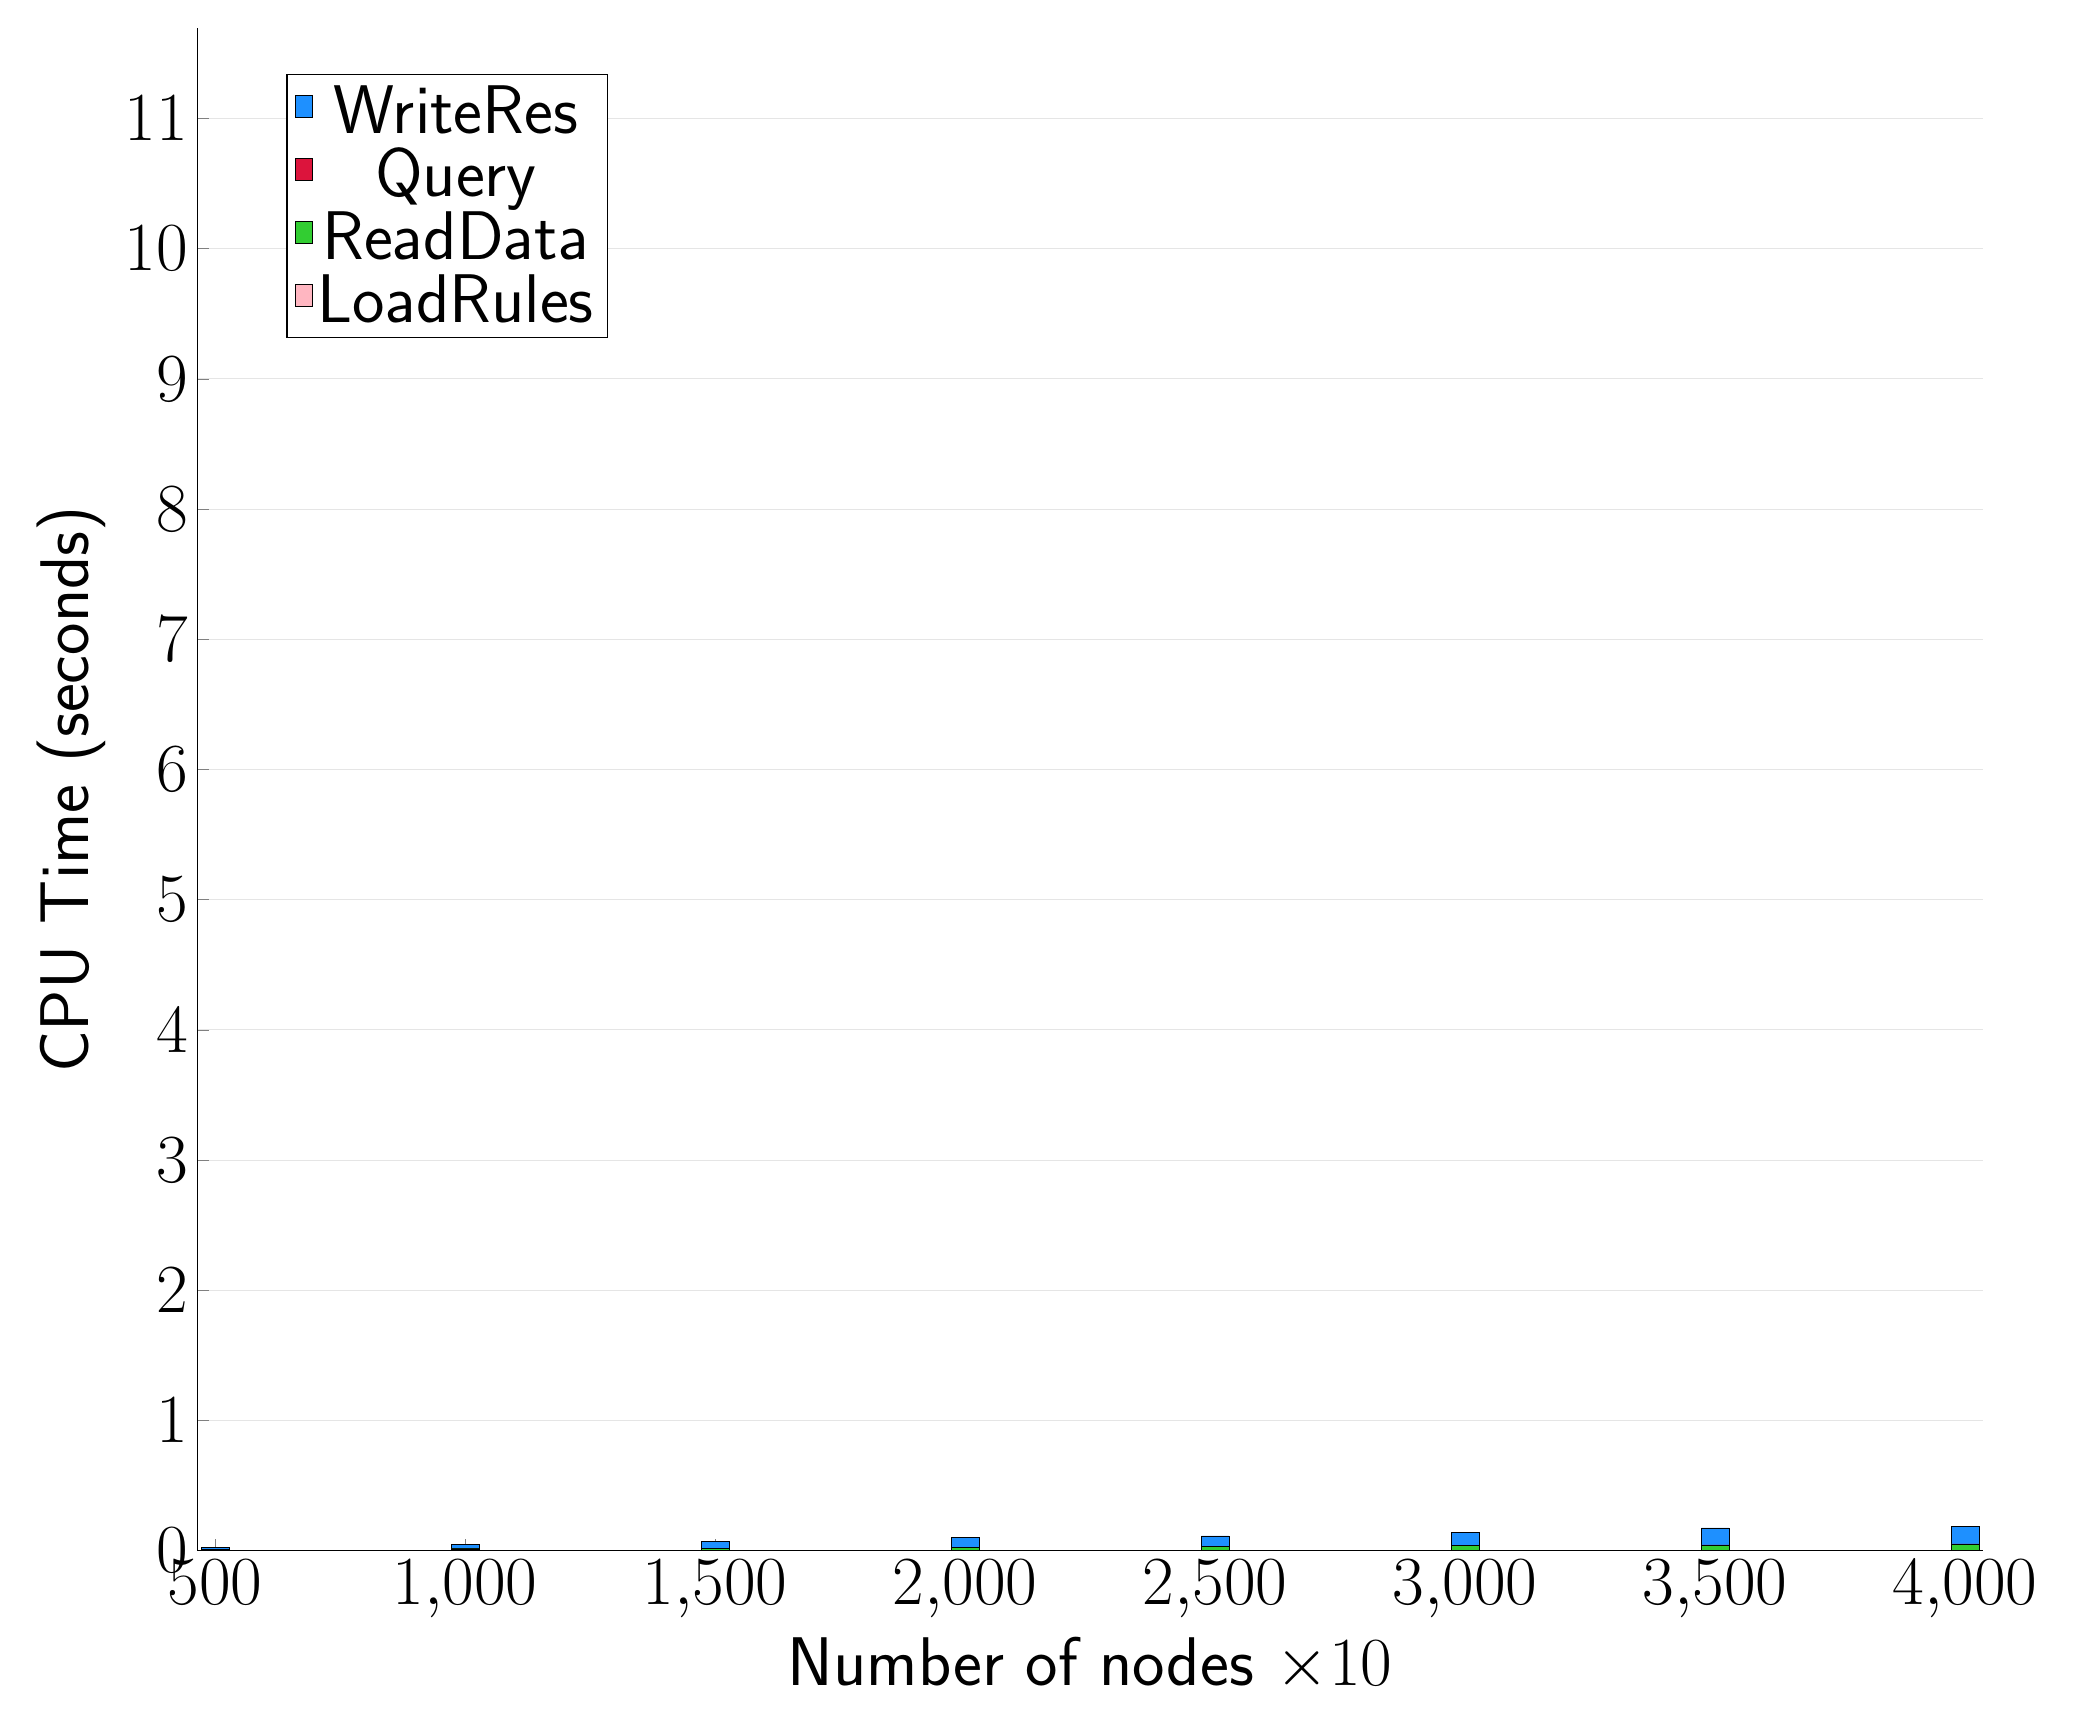
\begin{tikzpicture}
\begin{axis}[
   ybar stacked,
   width=2\textwidth,
   bar width=0.35cm,
   ymajorgrids, tick align=inside,
   major grid style={draw=gray!20},
   xtick=data,
   ymin=0, ymax=11.693333332737287,
   axis x line*=bottom,
   axis y line*=left,
   enlarge x limits=0.01,
   legend style={
       at={(0.23, 0.97)},
       anchor=north east,
       legend columns=1,
       font=\Huge,
   },
   ylabel={CPU Time (seconds)},
   xlabel={Number of nodes $\times 10$},
   label style={font=\Huge},
   tick label style={font=\Huge},
]
\addlegendimage{fill=DodgerBlue, draw=black, line width=0.2pt}
\addlegendentry{WriteRes}
\addlegendimage{fill=Crimson, draw=black, line width=0.2pt}
\addlegendentry{Query}
\addlegendimage{fill=LimeGreen, draw=black, line width=0.2pt}
\addlegendentry{ReadData}
\addlegendimage{fill=LightPink, draw=black, line width=0.2pt}
\addlegendentry{LoadRules}
\addplot +[fill=LightPink, draw=black, line width=0.2pt] coordinates {
(500, 0.0036773333333333332)
(1000, 0.002721333333333333)
(1500, 0.002425333333333334)
(2000, 0.0036076666666666666)
(2500, 0.003024)
(3000, 0.0032133333333333337)
(3500, 0.003251)
(4000, 0.0030779999999999996)
};
\addplot +[fill=LimeGreen, draw=black, line width=0.2pt] coordinates {
(500, 0.006654333333333334)
(1000, 0.011632666666666666)
(1500, 0.015775)
(2000, 0.02353066666666667)
(2500, 0.027585666666666665)
(3000, 0.03433733333333333)
(3500, 0.038688)
(4000, 0.046556999999999994)
};
\addplot +[fill=Crimson, draw=black, line width=0.2pt] coordinates {
(500, 0.00018966666666666936)
(1000, 0.00029099999999999965)
(1500, 0.0005363333333333354)
(2000, 0.0007926666666666663)
(2500, 0.0007770000000000011)
(3000, 0.0014613333333333334)
(3500, 0.0016293333333333368)
(4000, 0.0019020000000000068)
};
\addplot +[fill=DodgerBlue, draw=black, line width=0.2pt] coordinates {
(500, 0.017303333333333327)
(1000, 0.034654333333333336)
(1500, 0.05112866666666666)
(2000, 0.07234666666666667)
(2500, 0.08211666666666666)
(3000, 0.099814)
(3500, 0.13112333333333334)
(4000, 0.13222466666666668)
};
\end{axis}
\end{tikzpicture}

\end{document}
